\begin{figure}[htb]
    \centering   
    \begin{subfigure}[b]{0.24\textwidth}
        \centering
        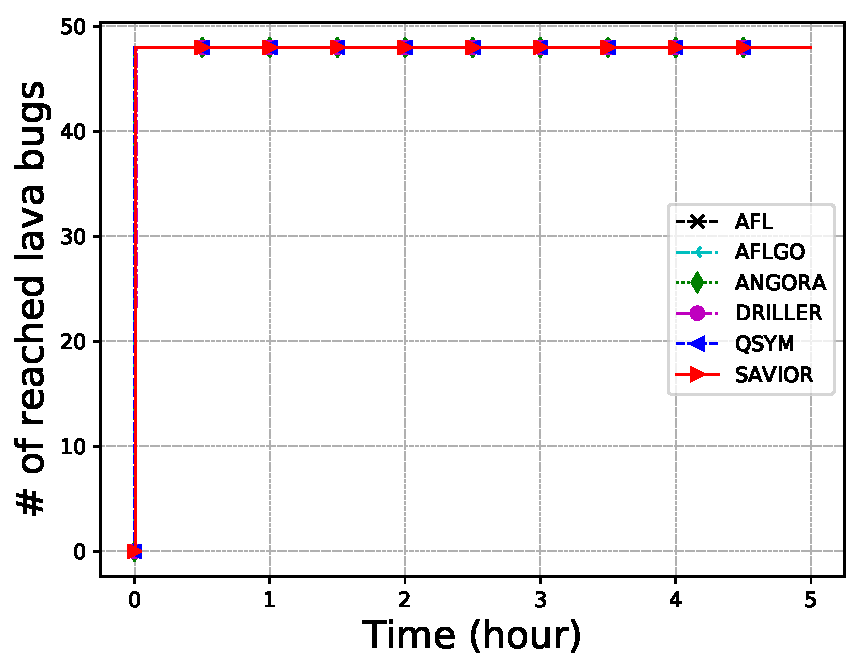
\includegraphics[width=1\textwidth]{savior/figures/lava_base64_bugcov.pdf}
        \caption{\scriptsize{Number of bugs reached in base64}}
        \label{fig:eval:lava:uniq}
    \end{subfigure}
        \begin{subfigure}[b]{0.24\textwidth}
        \centering
        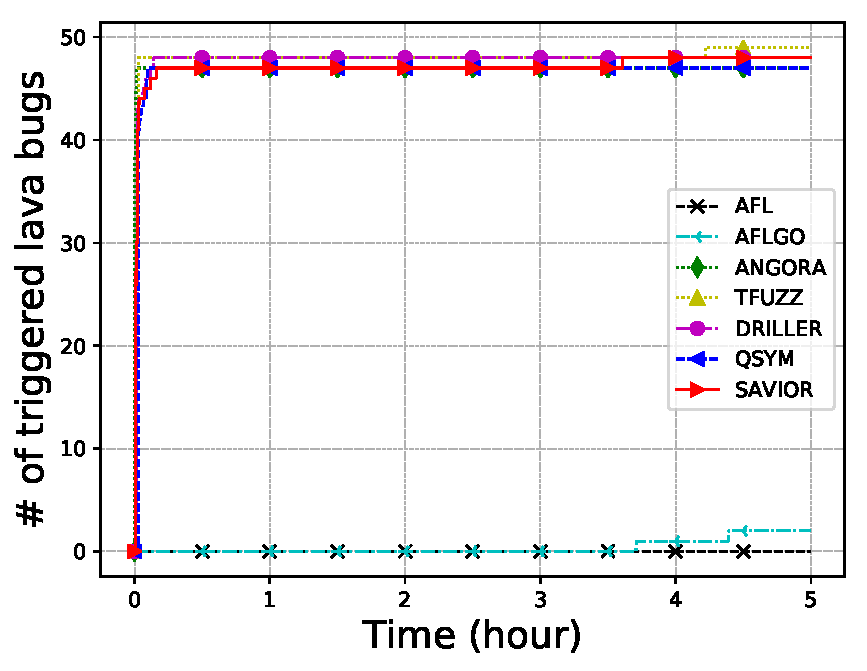
\includegraphics[width=1\textwidth]{savior/figures/lava_base64.pdf}
        \caption{\scriptsize{Number of bugs triggered in base64}}
        \label{fig:eval:lava:base64}
    \end{subfigure}\\
    \begin{subfigure}[b]{0.24\textwidth}
        \centering
        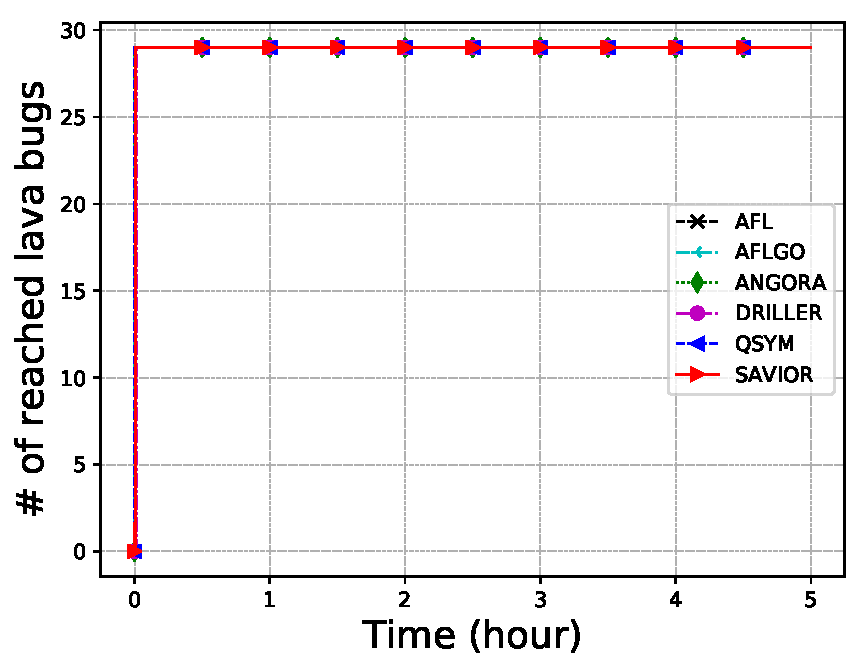
\includegraphics[width=1\textwidth]{savior/figures/lava_uniq_bugcov.pdf}
        \caption{\scriptsize{Number of bugs reached in uniq}}
        \label{fig:eval:lava:uniq}
    \end{subfigure}
    \begin{subfigure}[b]{0.24\textwidth}
        \centering
        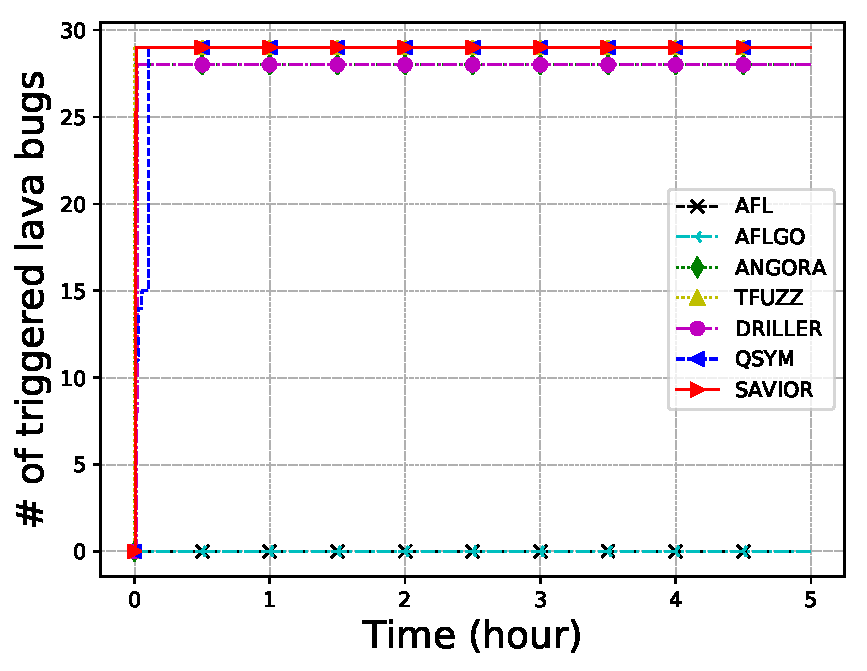
\includegraphics[width=1\textwidth]{savior/figures/lava_uniq.pdf}
        \caption{\scriptsize{Number of bugs triggered in uniq}}
        \label{fig:eval:lava:base64}
    \end{subfigure}\\
    \begin{subfigure}[b]{0.24\textwidth}
        \centering
        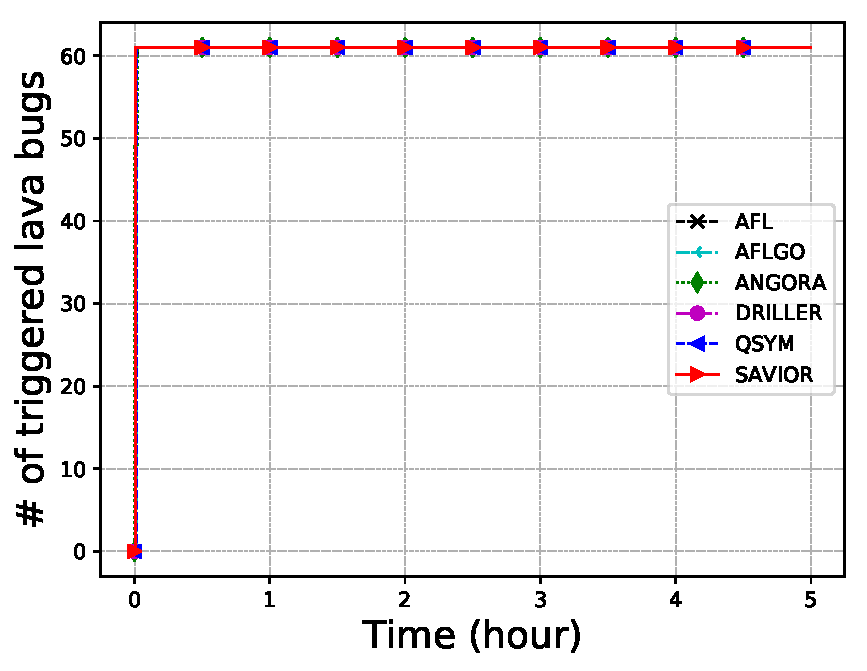
\includegraphics[width=1\textwidth]{savior/figures/lava_md5sum_bugcov.pdf}
        \caption{\scriptsize{Number of bugs reached in md5sum}}
        \label{fig:eval:lava:who}
    \end{subfigure}  
    \begin{subfigure}[b]{0.24\textwidth}
        \centering
        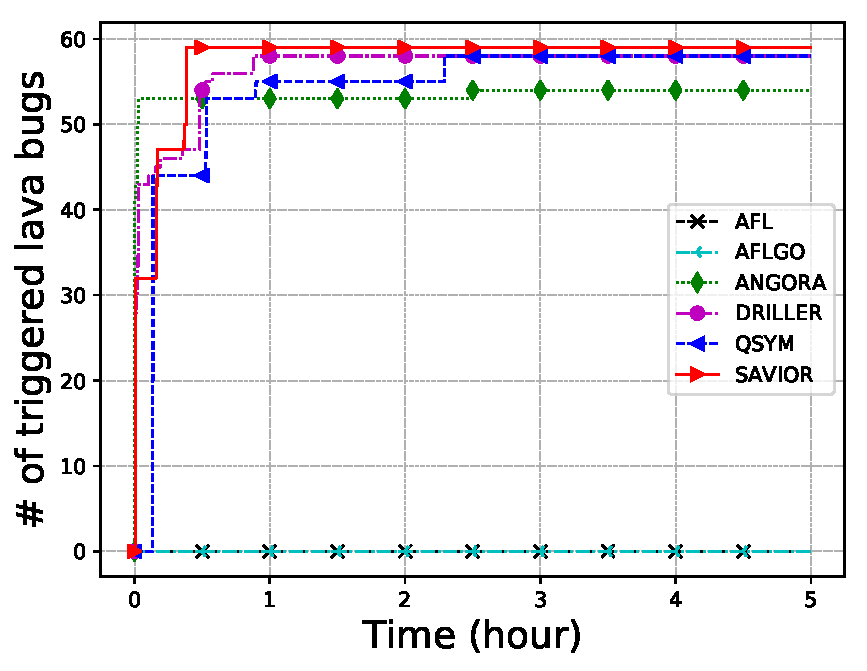
\includegraphics[width=1\textwidth]{savior/figures/lava_md5sum.pdf}
        \caption{\scriptsize{Number of bugs triggered in md5sum}}
        \label{fig:eval:lava:md5sum}
    \end{subfigure}\\
    \begin{subfigure}[b]{0.24\textwidth}
        \centering
        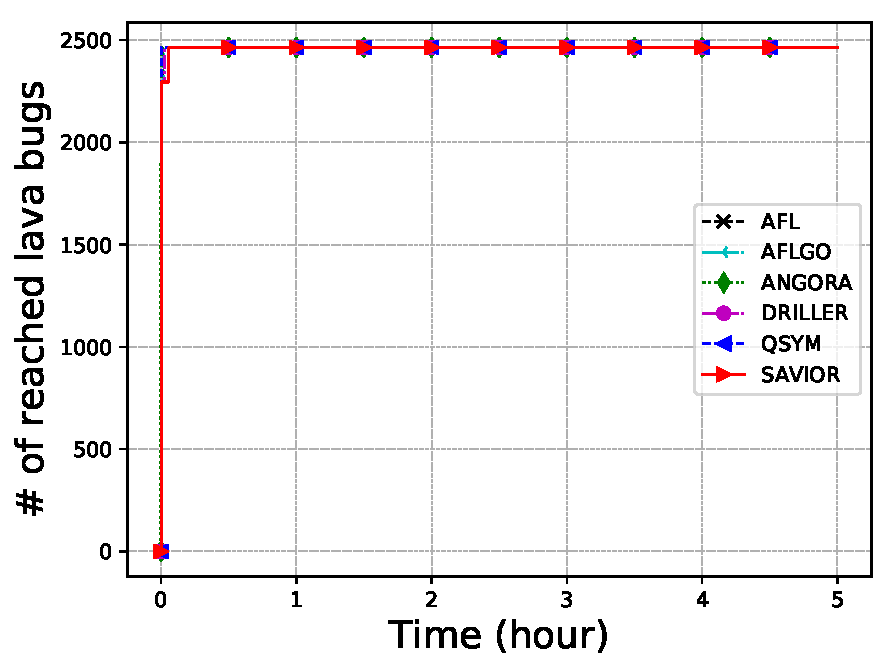
\includegraphics[width=1\textwidth]{savior/figures/lava_who_bugcov.pdf}
        \caption{\scriptsize{Number of bugs reached in who}}
        \label{fig:eval:lava:who}
    \end{subfigure}
    \begin{subfigure}[b]{0.24\textwidth}
        \centering
        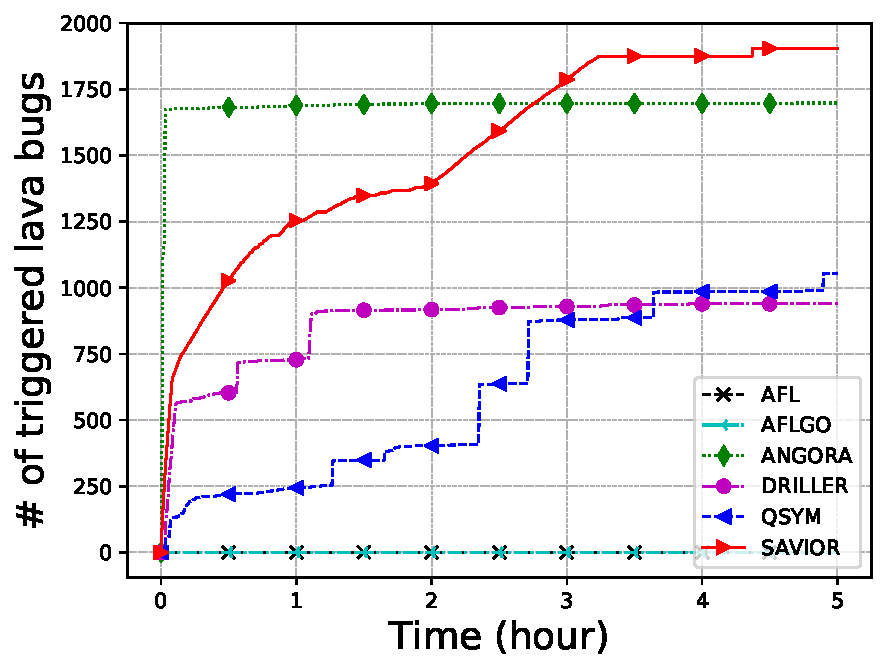
\includegraphics[width=1\textwidth]{savior/figures/lava_who.pdf}
        \caption{\scriptsize{Number of bugs triggered in who}}
        \label{fig:eval:lava:md5sum}
    \end{subfigure}
    \caption{Evaluation results with LAVA-M. The left column shows the number of reached lava-bugs by those fuzzers while the right column shows the number of lava-bug triggered by different fuzzers. For {\tt TFuzz}, we only present the number of triggered bugs in {\tt base64} and {\tt uniq}, as the other resutls are not reliable due to defects in a third-party component. This has been confirmed with the developers of {\tt TFuzz}.}
    \label{fig:lava_cfa}
\end{figure}





\subsection{Preliminary Results and Analysis}
\label{savior:sec:eval}

\subsubsection{Evaluation with LAVA-M}


\begin{table*}[h]
	\centering
		\caption{Fuzzer specific settings in evaluation with Lava-M.}
		\label{tab:lava-setup}
		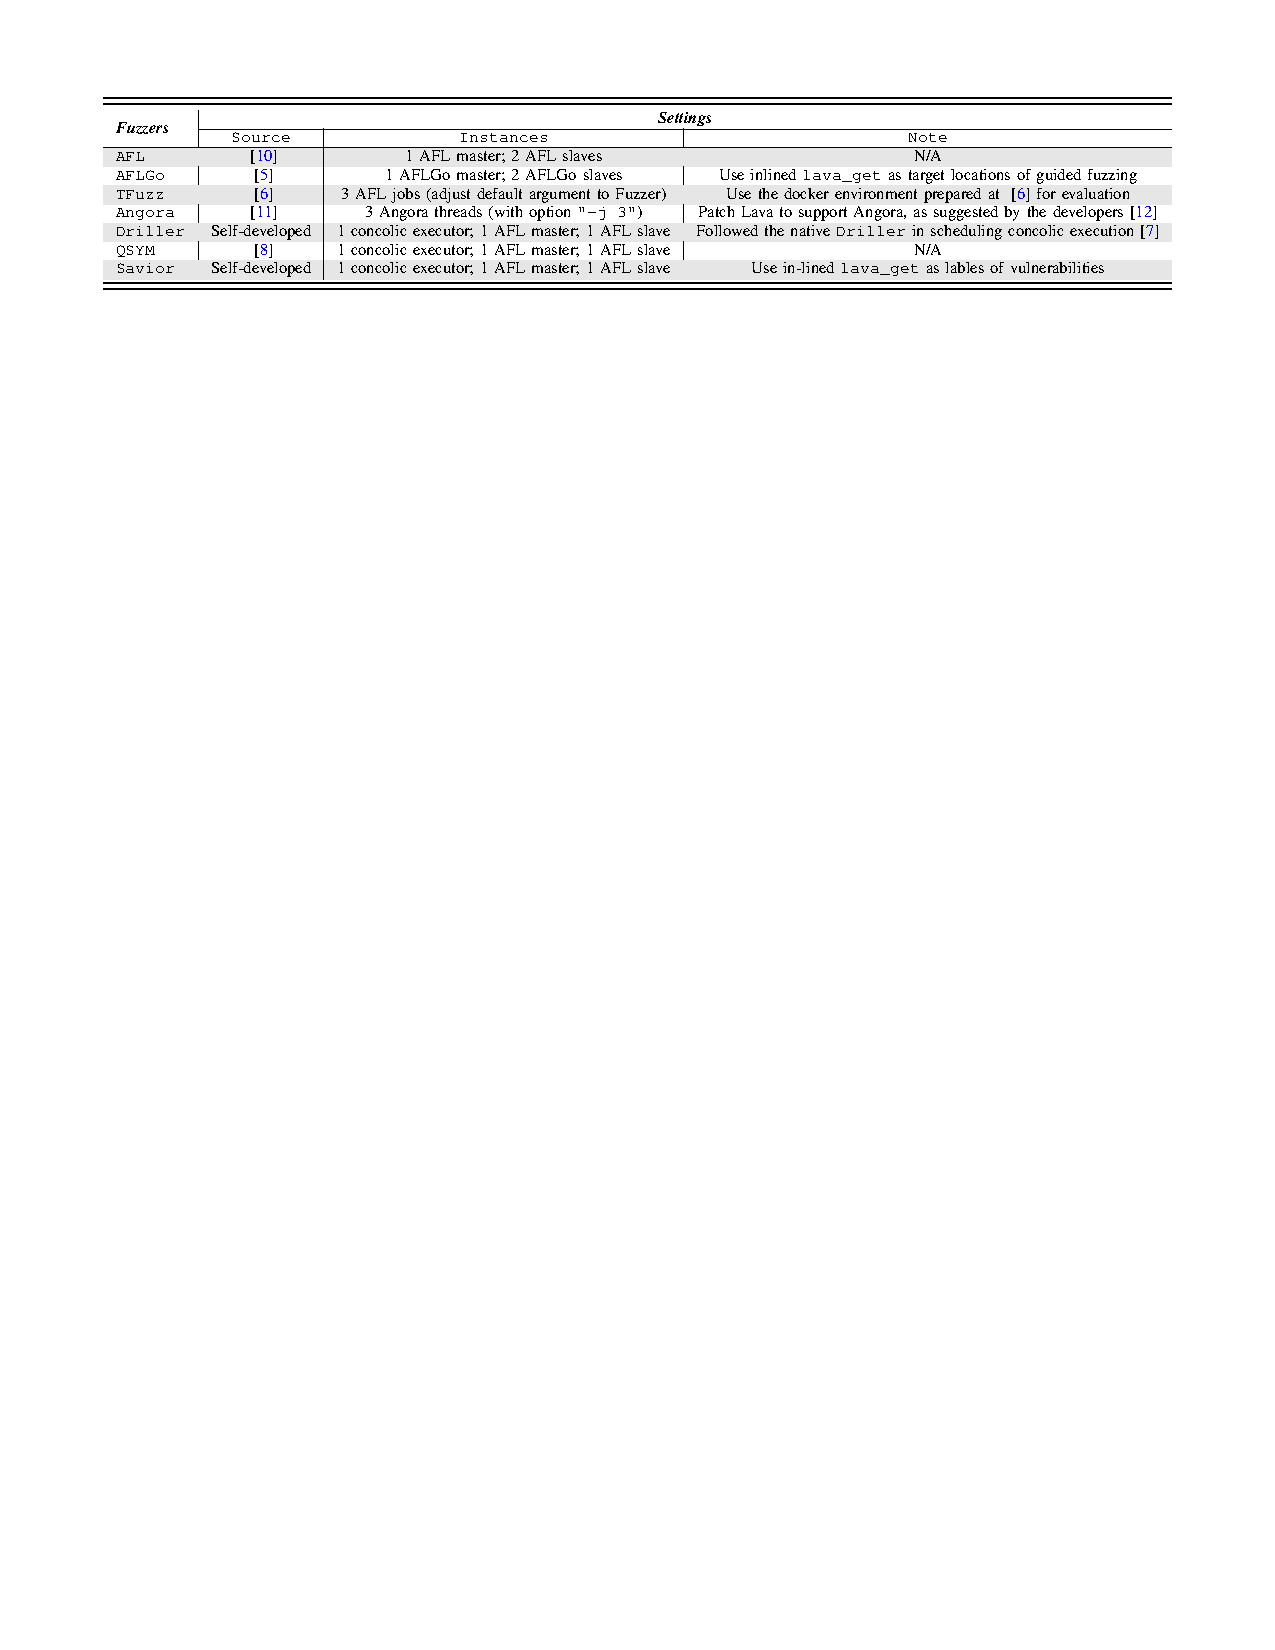
\includegraphics[scale=1]{savior/tables/lavasetup}
\end{table*}

\paragraph{Experimental Setup}
In this evaluation, we run each of the fuzzers in Table~\ref{tab:lava-setup} with four 
LAVA-M~\cite{lava} programs and we use the seeds shipped with the benchmark.  
For consistency, we conduct all the experiments on r4.16xlarge amazon EC2 instances 
with Ubuntu 16.04 LTS and we sequentially run all the experiments to avoid interference. 
In addition, we affiliate each fuzzer with 3 free CPU cores to ensure fairness with computation resources. 
Following the previous works~\cite{qsyminsu, angora,tfuzz}, we run each test for 5 hours.
To minimize the effect of randomness in fuzzing, we repeat each test 5 times and 
report the average results.
The settings specific to each fuzzer is summarized in Table~\ref{tab:lava-setup}, 
including how we distribute the 3 CPU cores and the actions we take to accommodate those fuzzers. 
In LAVA-M, each artificial vulnerability is enclosed in a function call to {\tt lava\_get} (in-lined in our evaluation).
We use these calls as the targets to guide {\tt AFLGo} and we mark them as vulnerability labels 
to enable bug-driven prioritization in \savior. In addition, as the vulnerability condition is 
hard-coded in the {\tt lava\_get} function, we naturally have support for bug-guided search.
Finally, for {\tt Angora}, we adopt the patches as suggested by the developers~\cite{tool-angora1}. 

\paragraph{Evaluation Results}In the left column of Figure~\ref{fig:lava_cfa}, 
we show how many vulnerabilities are reached over time by different fuzzers. The results demonstrate that all 
the fuzzers can instantly cover the code with LAVA vulnerabilities. However, as presented 
in the right column of Figure~\ref{fig:lava_cfa}, \tfuzz, \angora, \driller, \qsym, and \savior are able to 
trigger most (or all) of the vulnerabilities while \afl and \aflgo can trigger few. 
The reason behind is that the triggering conditions of LAVA vulnerabilities are all in the form of 
32-bit magic number matching. Mutation-based fuzzers, including AFL
and AFLGo, can hardly satisfy those conditions while the other fuzzers are all featured 
with techniques to solve them. 

Despite \tfuzz, \angora, \driller, \qsym, and \savior all trigger large numbers of LAVA vulnerabilities, 
they differ in terms of comprehensiveness and efficiency. \tfuzz quickly covers 
the listed vulnerabilities in {\tt base64} and {\tt uniq}. This is attributable to 
that (1) \tfuzz can reach all the vulnerabilities with the initial several seeds and (2) \tfuzz 
can transform the program to immediately trigger the encountered vulnerabilities.
Note that we do not show the results of \tfuzz on {\tt md5sum} and {\tt who},
because \tfuzz gets interrupted by a defective third-party component\footnote{This has been confirmed with the 
developers.}. For all the cases, \angora triggers most vulnerabilities
immediately after its start. The main reason is that the ``black-box function'' 
pertaining to all LAVA vulnerabilities 
is {\tt f(x) = x} and the triggering conditions are like {\tt f(x) == CONSTANT}. 
\angora always starts evaluates such functions with {\tt x = CONSTANT} and therefore, 
it can instantly generate seeds that satisfy the vulnerability conditions. 
In the case of {\tt who}, \angora does not make all the vulnerabilities 
because of the incomplete dynamic taint analysis. 

Regarding the three hybrid tools, they can trigger every vulnerability 
that their concolic executor encounters. In the cases of {\tt base64}, {\tt uniq}, and {\tt md5sum}, 
their concolic executor can reach all the vulnerabilities with (arbitrary) initial seeds,
which explains why the fuzzers all quickly trigger the listed vulnerabilities (regardless of their seed scheduling). 
But in the case of {\tt who}, even though the fuzzing component quickly generate
seeds to cover code containing vulnerabilities, 
it takes the concolic executor much longer to run those seeds.
For instance, while executing the inputs from \afl, \qsym needs 
around 72 hours of continuous concolic execution to reach 
all the LAVA vulnerabilities in {\tt who}. It's worth noting that \driller (with a random seed scheduling) 
moves faster than \qsym, because \qsym prioritizes concolic execution 
on small seeds, while reaching many vulnerabilities in {\tt who} needs larger seeds.

\begin{table*}[h]
	\centering
	\begin{minipage}[b]{0.45\textwidth}
		\centering	
		\caption{Bug triggered by different fuzzers in evaluation with Lava-M (with bug-guided search).}
		\label{tab:lava-bug-num}
		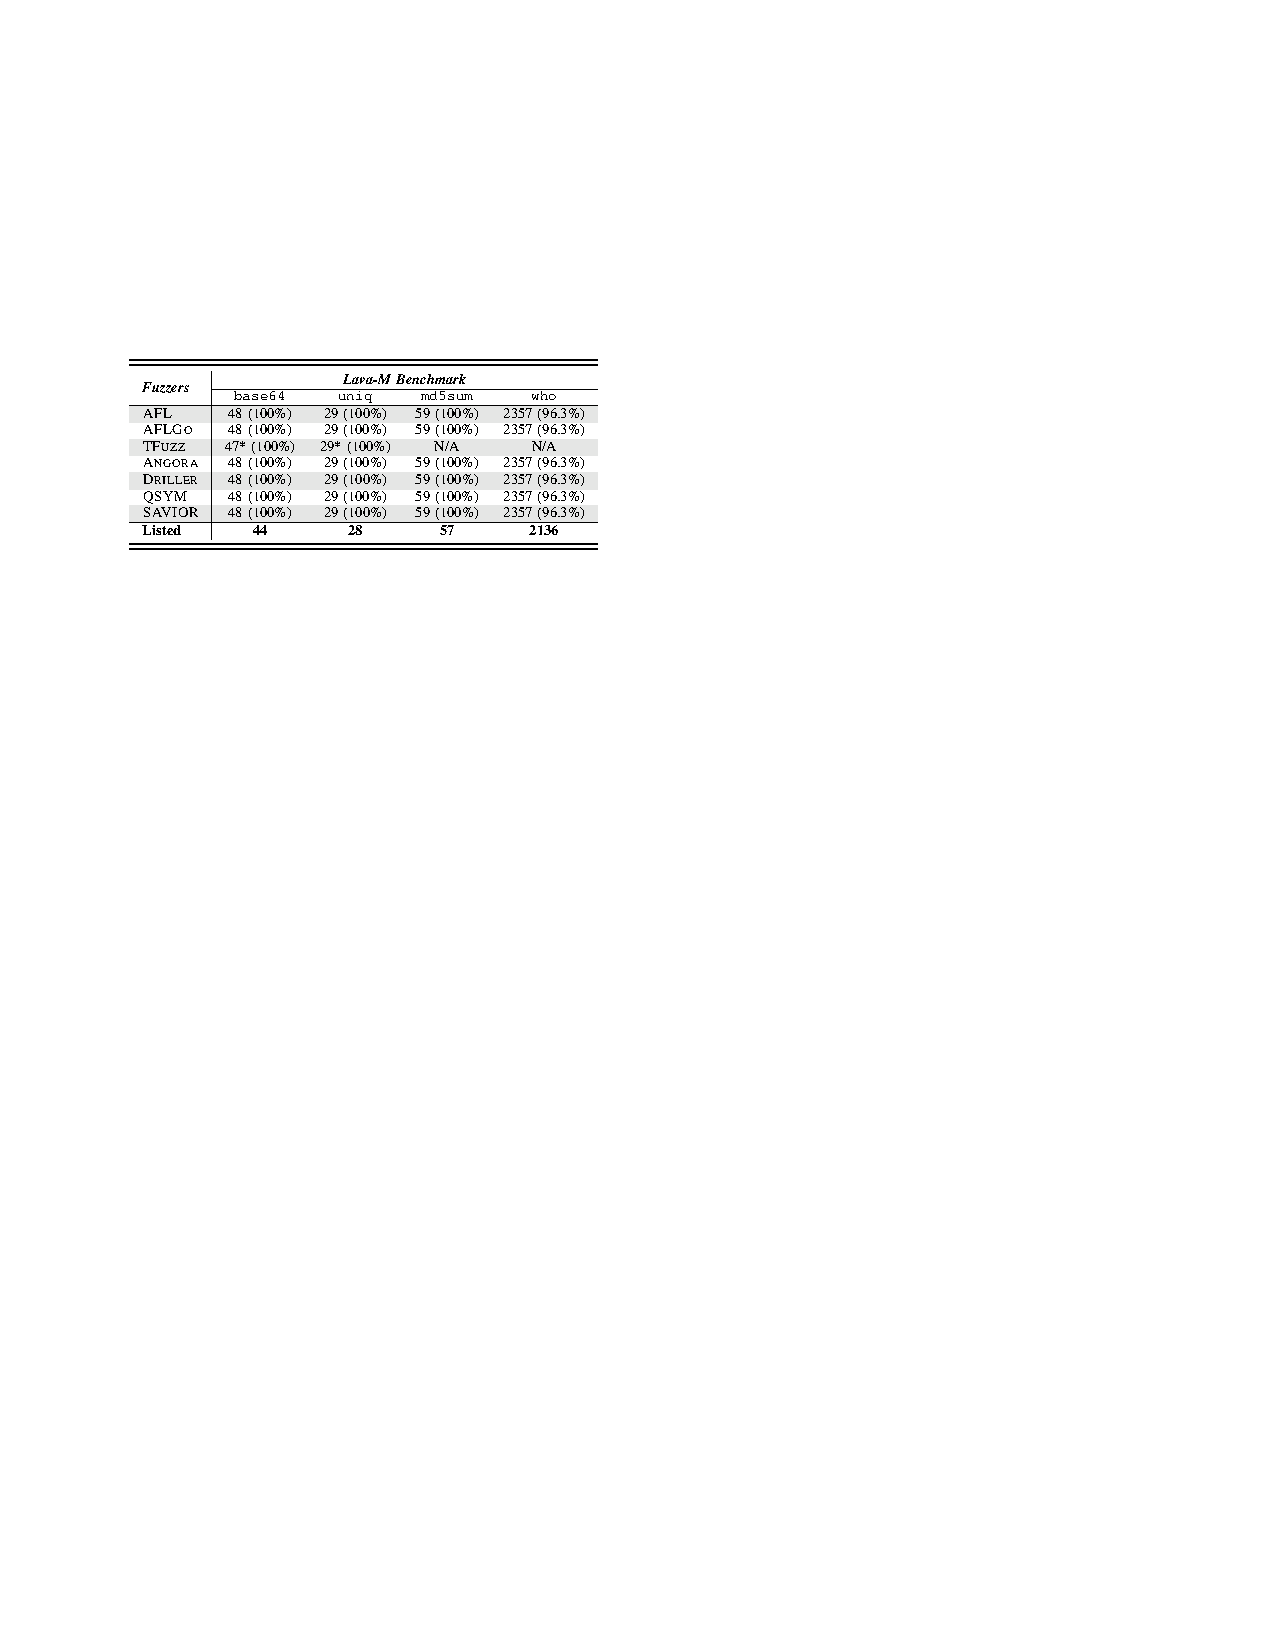
\includegraphics[scale=0.80]{savior/tables/bugguidedsearchlava}
	\end{minipage}
 	\hfill
	\begin{minipage}[b]{0.45\textwidth}
		\centering	
		\caption{IDs of Lava bugs that are not listed but identified by bug-guided search.}
		\label{tab:new-laval-bug-search}
		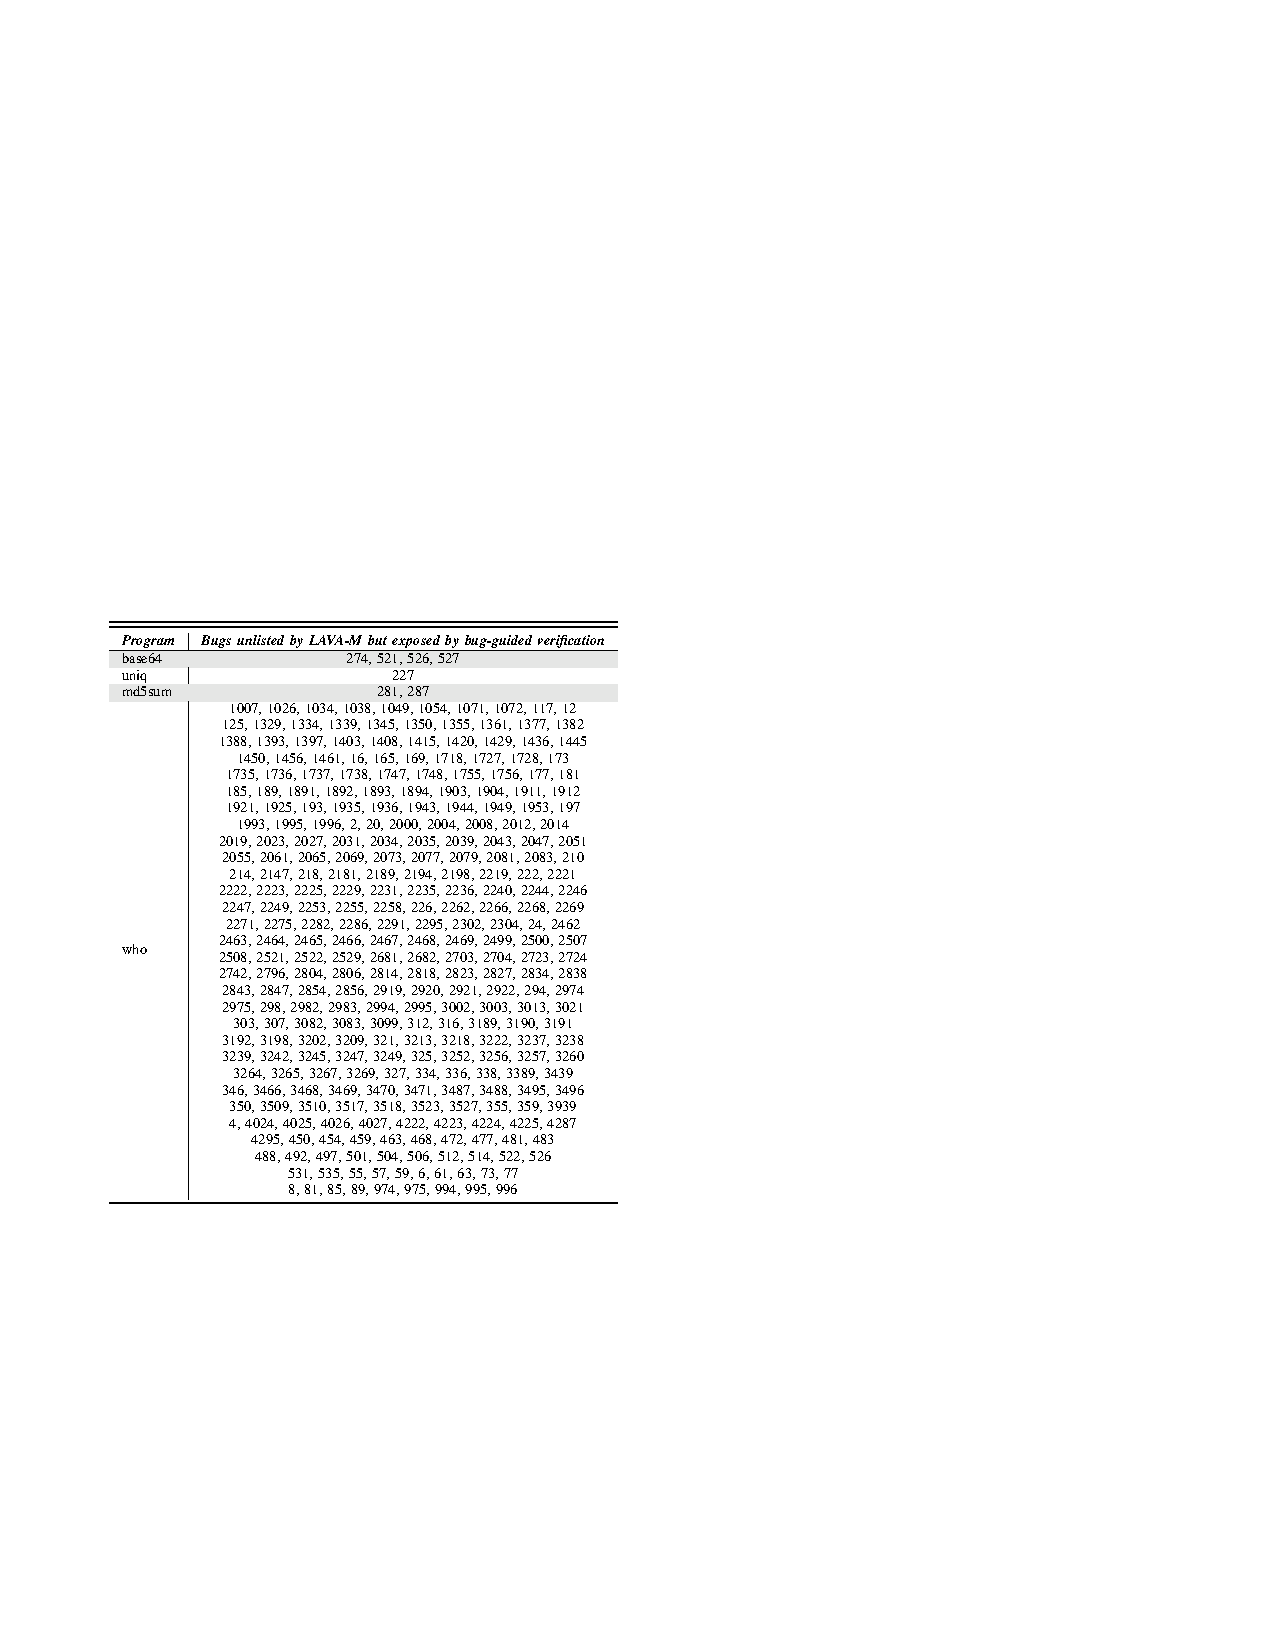
\includegraphics[scale=0.80]{savior/tables/unlistedlavabug}
	\end{minipage}
\end{table*}


As mentioned before, all the fuzzers have generated seeds to reach all the vulnerabilities, which they cannot 
trigger all of them either because their incapability to satisfy the conditions or because they did not finish 
concolic execution on all the seeds. We extended a further experiment by performing bug-guided searching with 
the seeds from all the fuzzers. Simply speaking, we run each of the seeds from all the fuzzers with the 
concolic executor in \savior. In this experiment, we only do constraint solving when a LAVA-M vulnerability condition
is encountered. This simulates the process of bug-guided search for all fuzzers. Enhanced with our bug-guided search, all the fuzzers 
can trigger not only the listed bugs in LAVA, as shown in Table~\ref{tab:lava-bug-num}, 
but also a group of unlisted bugs (Table~\ref{tab:new-laval-bug-search}). 






